\chapter{Fairness Through Regularization}
\label{ch:fairness_inproc}

% the integrated approach or in-processing

% \todo[inline]{changing the title to in-processing methods to achieve fairness?}
% \todo[inline]{accuracy or utility or personalization in general?}
As we discussed in Chapter \ref{ch:fairness}, there are three main approaches to integrating fairness notions into recommender systems: pre-processing, in-processing, and post-processing. Fairness integration through in-processing, is a topic of considerable research interest in recommender systems. Such algorithms treat recommendations as multi-objective optimization problems where the goal is to maintain a certain level of accuracy, while ensuring fairness in recommendation lists. One of the main challenges in doing so, is the inherent trade-off between personalization and non-accuracy metrics such as fairness that are incorporated in the objective function.

Personal preference is the essence of recommendation, where individual taste is paramount. As we explained in Chapter \ref{ch:fairness}, personalization and fairness are competing goals due to various reasons. Additionally, many recommendation applications involve multiple stakeholders, and each one may have fairness concerns of its own that might oppose other concerns. Therefore, for the multisided platforms to thrive, it is important to satisfy the fairness concerns of different stakeholders while maintaining personalization as a promised service to users.

In-processing methods are one approach to negotiate between fairness and accuracy. This section examines applications in which fairness with respect to consumers (C-fairness) and the providers (P-fairness) is important. We show that variants of the well-known sparse linear method (SLIM) can be used to achieve a reasonable balance between fairness and accuracy in collaborative filtering, and being in control of this balance. To improve ``fairness'' for, in the proposed method, we generate neighborhoods (i.e. all the users or items that are similar to each other in some way) for collaborative recommendations in such a way to have \textit{balanced representation} of the opinions across groups. We demonstrate that this method can be used for provider-side and consumer-side fairness.

% Note that, our goal is to achieve group fairness (consumer or provider) and will measure fairness of the results accordingly.
% One option that we explore in this paper is to design a recommender system following the approach of \cite{zemel2013learning} in generating fair classification. % A recommender system distinguished by C-fairness is one that must take into account the disparate impact of recommendation on protected classes of recommendation consumers.


\section{Balanced Neighborhoods in Recommendation}

The idea of creating a balanced representation to achieve fairness was first proposed by \cite{zemel2013learning}. In their work, the authors impose a fairness constraint on a classification by creating a set of prototypes to which instances are mapped, which are called as \textit{fair representations}. The prototypes each have equal representations of users in the protected and unprotected classes so that the association between an instance and a prototype carries no information about the protected attribute. 

As noted above, the requirement for personalization in recommendation means that we have as many classification tasks as we have users. A direct application of the fair prototype idea would aggregate many users together and produce the same recommendations for all, significantly reducing the level of personalization and the recommendation accuracy. This idea must be adapted to apply to recommendation where maintaining personalization is a goal. One of the fundamental ideas of collaborative recommendation is that of the \textit{peer user}, a neighbor whose patterns of interest match those of the target user and whose ratings can be extrapolated to make recommendations for the target user. One place where bias may creep into collaborative recommendation may be through the formation of peer neighborhoods.

Consider the situation in Figure~\ref{fig:neighbor}. The target user here is the solid square, a member of the protected class. The top of the figure shows a neighborhood for this user in which recommendations will be generated only from other square users, that is, other protected individuals. We can think of this as a kind of segregation of the recommendation space. If the peer neighborhoods have this kind of structure relative to the protected class, then this group of users will only get recommendations based on the behavior and experiences of users in their own group. For example, in a job recommendation example, women would only get recommendations of jobs that have interested other women applicants, potentially leading to very different recommendation experiences across genders. 

\begin{figure}[bh]
    \centering
    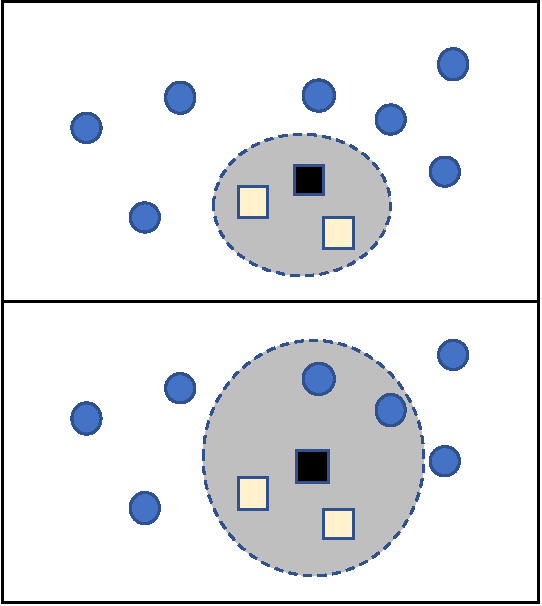
\includegraphics[width=1.5in]{imgs/bln/neighborhood.pdf}
    \caption{Unbalanced (top) and balanced (bottom) neighborhoods}
    \label{fig:neighbor}
\end{figure}

To enhance the degree of C-fairness in such a context, we introduce the notion of a \textit{balanced neighborhood}. A balanced neighborhood is one in which recommendations for all users are generated from neighborhoods that are balanced with respect to the protected and unprotected classes. This is shown in the bottom half of Figure~\ref{fig:neighbor}. The target has an equal number of peers inside and outside of the protected class. In the case of job recommendation, this would mean that female job seekers get recommendations from some female and some male peers.
% \todo[inline]{I have job recommendation examples here and there for the case of C-fairness, should I elaborate on that?}

There are a variety of ways that balanced neighborhoods might be formed. The simplest way would be to create neighborhoods for each user that balance accuracy against group membership. However, this would be highly computationally inefficient, requiring the solution of a separate optimization problem for each user. In this research, we explore an extension of the well-known Sparse Linear Method (SLIM)~\cite{ning2011slim}. SLIM is well-known as a state-of-the-art technology for collaborative recommendation. It is a generalization of item-based recommendation in which a regression coefficient is learned for each $\langle user, item \rangle$ pair. It can be slower to optimize than factorization-based methods, but for our purposes, it has the important benefit that the learned coefficients are readily interpretable with regard to group membership. Our extension of SLIM uses regularization to control the way different neighbors are weighted, with the goal of achieving balance between protected and non-protected neighbors for each user.
% \todo[inline]{how to interpret the slim coefficients for pro and unpro groups?}

\section{Sparse Linear Method}
% \hfill

SLIM learns $\langle user, item \rangle$ regression weights through optimization, minimizing a regularized loss function. Although this is not proposed in the original SLIM paper, it is possible to create a user-based version of SLIM (labeled SLIM-U in~\cite{zheng2014cslim}), which generalizes the user-based algorithm in the same way. 

% \todo[inline]{check the notations}
Assume that there are $M$ users (a set $U$), $N$ items (a set $I$), and let us denote the associated 2-dimensional rating matrix by $R$. SLIM is designed for item ranking and therefore $R$ is typically binary. We will relax that requirement in this work, we use $u_i$ to denote user $i$ and $t_j$ to denote the item $j$. An entry, $r_{ij}$, in matrix $R$ represents the rating of $u_i$ on $t_j$. SLIM-U predicts the ranking score $\hat{s}$ for a given user, item pair $\langle u_i, t_j \rangle$ as a weighted sum:

\begin{equation}
    \hat{s}_{ij} = \sum_{k \in U}{w_{ik}r_{kj}}, 
\end{equation}
where $w_{ii} = 0$ and $w_{ik} >= 0$.
\vspace{0.25cm}

Alternatively, this can be expressed as a matrix operation yielding the entire prediction matrix $\hat{S}$:    
\begin{equation}
\hat{S} = WR,
\end{equation}
\vspace{0.25cm}

where $W$ is an $M \times M$ matrix of user-user weights. For efficiency, it is very important that this matrix be sparse.

The optimal weights for SLIM-U can be derived by solving the following minimization problem:

\begin{equation}
\text{min}_W~\frac{1}{2}\left\Vert R - WR \right\Vert^2 + 
    \lambda_1 \left\Vert W \right\Vert^1 +
    \frac{\lambda_2}{2}\left\Vert W \right\Vert^2,   
\end{equation}
subject to $W > 0$  and $\text{diag}(W) = 0$.
\vspace{0.25cm}


The $\left\Vert W \right\Vert^1$ represents the $\ell_1$ norm and the $\left\Vert W \right\Vert^2$ term represents the $\ell_2$ norm of the $W$ matrix. These regularization terms are present to constrain the optimization to prefer sparse sets of weights. Typically, coordinate descent is used for optimization. Refer to \cite{ning2011slim} for additional details. 

% \todo[inline]{subsubsection? or paragraph?}
\subsection{Neighborhood Balance}
% \paragraph{\textbf{Neighborhood Balance}}

Recall that our aim in fair recommendation is to eliminate segregated recommendation neighborhoods where protected class users only receive recommendations from other users in the same class. Such neighborhoods would tend to magnify any biases present in the system. If users in the protected class only are recommended certain items, then they will be more likely to click on those items, and thus increase the likelihood that the collaborative system will make these items the ones that others in the protected group see.

To reduce the probability that such neighborhoods will form, we use the SLIM-U formalization of the recommendation problem, but we add another regularization term to the loss function, which we call the \textit{neighborhood balance} term. To describe this term, we will enrich our notation further by indicating $U^+$ to be the subset of $U$ containing users in the protected class with the remaining users in the class $U^-$. Let $W_i^+$ be the set of weights for users in $U^+$ and $W_i^-$ be the corresponding set of weights for the non-protected class. Then the neighborhood balance term $b_i$ for a given user $i$ is the squared difference between the weights assigned to peers in the protected class versus the unprotected class.

\begin{equation}
    b_i = (\sum_{w^+ \in W_i^+}{w^+} - \sum_{w^- \in W_i^-}{w^-})^2
\end{equation}
\vspace{0.25cm}

A low value for the neighborhood balance term means that the users' predictions will be generated by weighting protected, and unprotected users on a relatively equal basis. Note that this is a class-blind optimization that tries to build balanced neighborhoods for protected and unprotected users. It is also possible to formulate the objective such that it only impacts the protected class, and we leave this option for future work.

Another way to express this idea is to create a vector $p$ of dimension $M$. If $u_i$ is in $U^+$, then $p_i = 1$; if $u_i$ is in $U^-$, then $p_i = -1$. Then, the sum expressed above can be rewritten as $b_i = (p^T \cdot w_i)^2$. By adding up this term for all users and adding it to the loss function, we can allow the optimization process to derive weights with neighborhood balance in mind. This adapted version of SLIM-U we will call \textit{Balanced Neighborhood} SLIM-U or BN-SLIM-U. As in the case of the original SLIM implementation, we can apply the method of coordinate descent to optimize the objective. The full loss function is as follows:

\begin{equation}
\begin{split}
 L = \frac{1}{2}\left\Vert R - WR \right\Vert^2 + 
    \lambda_1 \left\Vert W \right\Vert^1 + 
    \frac{\lambda_2}{2}\left\Vert W \right\Vert^2 +
    \frac{\lambda_3}{2}\sum_{i \in U}\left(\sum_{k \in U}p_iw_{ik}\right)^2,
\end{split}
\end{equation}
\vspace{0.25cm}

where $w_{ii}=0$ and $w_{ik}>=0$ and where $\lambda_3$ is a parameter controlling the influence of the neighborhood balance calculation on the overall optimization

This loss function retains the property of the original SLIM algorithm in that the rows of the weight matrix are independent, and the weights in each row (those for each user) can be optimized independently. The algorithm chooses one $w_{ik}$ weight and solves the optimization problem for that weight, repeating over all the weights until convergence is reached. If we take the derivative of $L$ with respect to a single weight $w_{ik}$, we obtain

\begin{equation}\label{eq:derivative}
\begin{split}
\frac{\partial L_i}{\partial w_{ik}} = \sum_{j \in I}{(r_{ij} - 
    \sum_{l \in U'}{w_{il}r_{lj}})} + w_{ik}\sum_{j \in I}{r_{kj}^2} + 
    \lambda_1 + \lambda_2w_{ik} + \lambda_3p_k\sum_{l \in U'}{p_lw_{il}} 
\end{split}
\end{equation}
where $U' = U - \{u_i, u_k\}$.
\vspace{0.25cm}

We then set this derivative to zero and solve for the value of $w_{ik}$ that produces this minimum. This becomes the coordinate descent update step. 

\begin{equation}\label{eq:update}
\begin{split}
    w_{ik} \leftarrow \frac{S\left(X_{ik}, \lambda_1\right)_+}
    {\sum_{j \in I}{r_{kj}^2} + \lambda_2 + \lambda_3} \\ \\
    X_{ik} = \sum_{j \in I}{(r_{ij} - 
    \sum_{l \in U'}{w_{il}r_{lj}})}+\lambda_3p_k\sum_{l \in U'}{p_lw_{il}}\\
\end{split}
\end{equation}
where $S()_+$ is the soft threshold operator defined in ~\cite{friedman_pathwise_2007}.
\vspace{0.25cm}

\subsection{Item-based Neighborhoods}
% \paragraph{\textbf{Item-based neighborhoods}}

As noted above, some applications may require P-fairness: making the recommendation outcomes fair relative to the (item) providers being recommended.  In Kiva, the operators of this site aim to provide equal exposure to loans from different geographic regions. To address the P-fairness case, we can use an analogous approach using item neighborhoods and item weights, ensuring that items in a protected group are in neighborhoods that have balanced membership of items from the unprotected group. The derivation of the loss function is exactly analogous, yielding another variant of the SLIM algorithm that we refer to as \textit{Balanced Neighborhood} SLIM or BN-SLIM.

\section{Methodology}

% \todo[inline]{review and shrink as already discussed}
To evaluate our balanced neighborhood approach, we conducted separate sets of experiments for both consumer- and provider- fairness cases. It is very difficult to find datasets containing the kind of features that would be necessary to evaluate fairness-aware recommendation algorithms, especially related to user demographics in sensitive application areas such as employment. For the purposes of this project, we are using the well-known MovieLens 1M dataset~\cite{movielens}, which contains gender information for each user, as well as ratings of 4,000 movies by 6,000 users. For more details refer to \ref{ch:methodology}.
% \todo{label the sections in methodology}

% Movie recommendation is, of course, a domain of pure individual taste and therefore not an obvious candidate for fairness-aware recommendation. Following the example of \cite{yao2017beyond}, our approach to construct an artificial equity scenario within this data for expository purposes only, with the understanding that real scenarios can be approached with a similar methodology. 

\subsection{Consumer Fairness}

Our consumer-fairness scenario centers on movie genres since we could detect discrepancies in recommendation delivery to male and female users despite the similar rating behavior of both groups. Therefore we choose gender as the sensitive attribute with females as the protected and the males as the unprotected groups.

% It can be seen in this data that there is a minority of female users (1709 out of the total of 6040). Certain genres display a discrepancy in recommendation delivery to male and female users. For example, in the ``Crime'' genre, female users rate a very similar number of movies (average of 0.048\% of female profiles vs 0.049\% of male profiles) and rate them similarly: an average rating of 3.7 for both female and male users. However, our baseline unmodified SLIM-U algorithm recommends in the top 10 an average of 1.10 ``Crime'' movies per female user as opposed to 1.18 such movies to male users. We are still exploring the cause of this discrepancy, but it seems likely that there are influential female users with a lower opinion of this genre. 

% Given that the rating profiles are similar but the recommendation outcomes are different, we can therefore conclude that the female users experience a deprivation of ``Crime'' movies compared to their male counter-parts. Similar losses can be observed for other genres. We are not asserting that there is any harm associated with this outcome. It is sufficient that these differences allow us to validate the properties of the BN-SLIM-U algorithm.

Our goal, then, is to reduce or eliminate genre discrepancies with minimal accuracy loss by constructing balanced neighborhoods for MovieLens users. The $p$ vector in Equation~\ref{eq:update} therefore will have a $1$ for female users and a $-1$ for male users. The experiments below compare the user-based SLIM algorithm in its unmodified form and the balanced neighborhood version BN-SLIM-U. In evaluating fairness of outcome, here we measure \textit{relative opportunity}, explained in \ref{ch:methodology} which is the observed probability of protected class items being recommended divided by the probability of unprotected class items being recommended.

% \todo[inline]{refer to the methodology section again}
Based on this concept, we create a consumer-side equity score $E_c@k$ for recommendation lists of k items, as the ratio between the outcomes for the different consumer groups. In our MovieLens experiments, we measure the number of movies in protected and unprotected genres included in recommendation lists as the measure of outcome quality. 

% We construct a consumer-side equity score, $E_c@k$ for recommendation lists of k items, as the ratio between the outcomes for the different groups. Let $P_i@k = {\rho_1, \rho_2, ..., \rho_k}$ be the top $k$ recommendation list for user $i$, and let $\gamma()$ be a function $\rho \rightarrow \{0,1\}$ that maps to 1 if the recommended movie is in a protected genre. Then:

% \begin{equation}
% E_c@k=\frac{\sum_{i \in U^+}{\sum_{\rho \in P_i@k}{\gamma(\rho)}}/|U^+|}
% {\sum_{i \in U^-}{\sum_{\rho \in P_i@k}{\gamma(\rho)}}/|U^-|}
% \end{equation}

$E_c@k$ will be less than 1 when the protected group is, on average, recommended fewer movies of the desired genre. And higher $E_c@k$ means that the recommendation algorithm is, on average, providing more movies in the given genre to the protected group (reversing the unfairness). As in any multi-criteria setting, we must be concerned about any loss of accuracy that results from taking additional criteria into consideration. Therefore, we also evaluate the ranking accuracy of our algorithms in the results below. The measure that we use is normalized discounted cumulative gain (NDCG) measured at a specific list length. For more details please refer to \ref{ch:methodology}.


% It may be unrealistic to imagine that this value should approach 1: the metric does not correct for other factors that might influence this score -- for example, female users may rate a particular genre significantly lower and an equality of outcome should not be expected. % While the absolute value of the metric may be difficult to interpret, it is still useful for comparing algorithms. 

% The one with the higher $E_c@k$ is providing more movies in the given genre to the protected group. Note that this is an additive, utilitarian measure of outcome equity and does not take into account variations in user experience. More nuanced measures of distributional equity, including Pareto improvement, we leave for future work.


% In this measure, an item appearing on a recommendation list accrues ``gain'' according to its position on the list -- thus the discount. The measure is normalized by comparing the algorithm's performance to the best ranking that could have been achieved. 

% Let $P_i@10$ be a list of retrieved list of length 10 and let $\tau$ be an indicator function that is 1 for movies that the user liked and 0 for others. Then, DCG@10 is computed as

% \begin{equation}
% DCG@10 = \sum_{k=1}^{10}{\frac{\tau(\rho_k)}{log_2(k+1)}}
% \end{equation}

% NDCG@10 is this DCG@10 value divided by the optimal DCG, which occurs when all of the movies liked by the user and appearing the test set are ranked at the top of the list in their order of preference.

\subsection{Provider Fairness}
% \paragraph{\textbf{Provider fairness}}

To evaluate our approach for provider fairness, we are using the Kiva\footnote{http://build.kiva.org/} dataset (described in Chapter \ref{ch:methodology}). We find that there are some geographic regions with a higher than the average number of unfunded loans. In these regions, borrowers have a lower probability of getting the desired capital. See Table~\ref{tab:unfunded}.


% a dataset extracted from the Kiva.org microlending site using the site's API\footnote{http://build.kiva.org/}. Again, we have constructed our own scenario using this data, focusing on geographic region. In our dataset, we find that there are some geographic regions with a higher than average number of unfunded loans. In these regions, borrowers have a lower probability of getting the desired capital. See Table~\ref{tab:unfunded}.

% \todo[inline]{remove since it's in the methodology section}
% \begin{table}
%     \centering
% \begin{tabular}{l|l|r}
%     Category & Region & Unfunded \% \\ \hline
%     Unprotected & North America & 1.73 \\
%     & Eastern Europe & 0.99 \\
%     & South America & 4.33 \\
%     & Asia & 6.70 \\ \hline
%     Protected & Africa & 10.57 \\
%     & Middle East & 13.23 \\
%     & Central America & 8.81 \\
% \end{tabular}
%     \caption{Percentage of unfunded loans by region}
%     \label{tab:unfunded}
% \end{table}

% For the purposes of our experiments, we will assume that one of the goals of a microlending site is to equalize access to capital across geographic regions. Kiva does not currently offer personalized recommendation of loans to its users, but if it did, a fairness-aware recommendation approach could be used to promote the loans of borrowers in the underserved regions. 

Therefore we will treat the under-represented regions collectively as the protected group and the other regions as the unprotected group. This enables us to use our item-based neighborhood balance algorithm described above. A more fine-grained approach to geographic equity that tries to balance across all regions would require additional algorithmic development and is left for future work. Further, we will represent fairness as a ratio of outcomes. It is simpler to compute in this case, as we are not dividing the recommendations by genre. The provider-side equity score, $E_p@k$, is defined on recommendation lists of k items (explained in Chapter \ref{ch:methodology}). 


% Let $L^+$ be the set of loans in the test set that are from the protected regions, and $L^-$ be the corresponding set from the unprotected regions. Also, let $\pi^+()$ be an indicator function $\rho \rightarrow \{0,1\}$ that maps to 1 if the recommended loan is from a protected region and $\pi^-$ is a similar function for the unprotected regions. Then:

% \begin{equation}
% E_p@k=\frac{\sum_{i \in U}{\sum_{\rho \in P_i@k}{\pi^+(\rho)}}/|L^+|}
% {\sum_{i \in U}{\sum_{\rho \in P_i@k}{\pi^-(\rho)}}/|L^-|}
% \end{equation}

$E_p@k$ will be less than 1 when loans from the protected regions appear less often on recommendation lists. As with $E_c$, this is a utilitarian measure, summing over all borrower regions without considering the distribution across individual borrowers. Like $E_c$, it does not take the rank of recommended items into account.


\section{Results}

We implemented the SLIM-U, BN-SLIM, and BN-SLIM-U algorithms using LibRec 3.0~\cite{guo2015librec} and incorporated it in \libauto{} explained in Chapter \ref{ch:librec-auto}, and used its existing implementation of SLIM. We used 5-fold cross-validation as implemented within the library.

\subsection{Consumer Fairness: MovieLens}

Within the MovieLens 1M dataset, we selected the five genres on which the SLIM-U algorithm produced the lowest equity scores: ``Film-Noir'', ``Mystery'', ``Horror'', ``Documentary'', and ``Crime''. The parameters were set as follows: $\lambda_1 = 0.1$, $\lambda_2 = 0.001$, and (for BN-SLIM-U) $\lambda_3 = 25$. Because the balance term measures the difference in weights, it tends to be much smaller than the terms that measure the sums of weights. Therefore, the regularization constant must be much higher for the balance term to have an impact on the optimization. 

\begin{figure}[tbh]
    \centering
    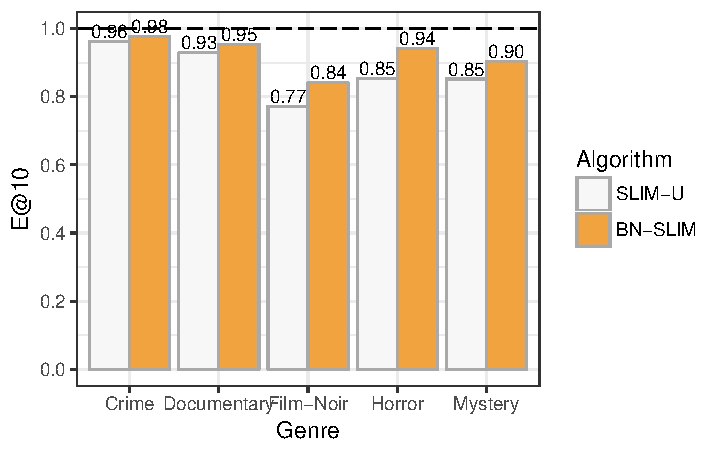
\includegraphics[width=3.00in]{imgs/bln/genre-compare3.pdf}
    \caption{Equity score for SLIM-U and BN-SLIM-U. Line indicates equal percentage across genders}
    \label{fig:genre}
\end{figure}

Figure~\ref{fig:genre} shows the results of the experiment in terms of the equity scores for each genre. Perfect equity (1.0) is marked with the dashed line. As we can see, in every case, the balanced neighborhood algorithm produced an equity score closer to 1.0 than the unmodified algorithm. The most significant jump is observed in the ``Horror'' genre, about 0.09 in the equity score or around 10\%. In terms of accuracy, there was only a small loss of NDCG@10 between the two conditions. See Table~\ref{tab:ndcg}. The difference amounts to approximately 2\% loss in NDCG@10 for the balanced neighborhood version.

\begin{table}
\centering
\begin{tabular}{c|c}
    Algorithm &  NDCG@10 \\ \hline
    SLIM-U & 0.053 \\ \hline
    BN-SLIM & 0.052 \\ \hline
\end{tabular}
\caption{Ranking accuracy}
\label{tab:ndcg}
\end{table}

Because the balanced neighborhood algorithm is applied across all users, it also shows male users movie genres that occur more frequently for female users. To see this effect, we examined the five genres with the highest $E_c@10$ values: ``Fantasy'', ``Animation'', ``War'', ``Romance'', and ``Western'' using the same parameter values as above. The results appear in Figure~\ref{fig:inverse-equity} and show a similar result. ``War'' is something of an anomaly here, both because it is perhaps unexpected to see it as a one of the more female-recommended genres and because the genre-balance algorithm pushes it to become more skewed rather than less. We investigated the cause of this phenomenon. Overall, the BN-SLIM-U algorithm produces a recommendation experience in which the occurrence of gender-specific genres is more closely equalized, with small loss in ranking accuracy.

\begin{figure}[bth]
    \centering
    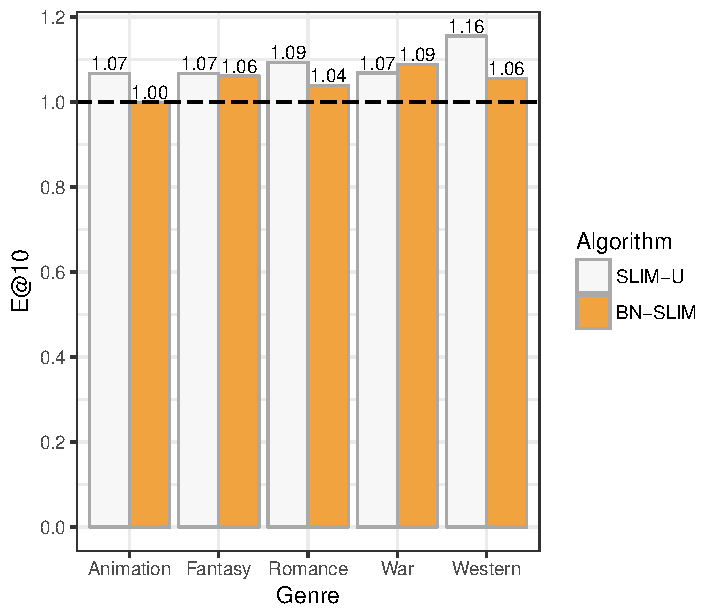
\includegraphics[width=3in]{imgs/bln/inverse-genres3.pdf}
    \caption{Equity scores for female-preferred genres}
    \label{fig:inverse-equity}
\end{figure}

\subsection{Provider Fairness: Kiva.org}

% Our dataset was extracted from Kiva's public API in September of 2016 and contains approximately 1 million loans funded by approximately 180,000 lenders. One challenge for collaborative recommendation in the microlending area is that loans are generally one-time endeavors. Unlike a movie that can be watched by an unrestricted number of viewers, a loan -- once funded -- disappears from Kiva.org and is not available for other lenders to view or support. Most loans are supported by from 1-330 lenders, by contrast, a popular movie in the MovieLens dataset might be rated by thousands of users. Thus, the lender-borrower relation is highly sparse, and loans have very small profiles.

% \todo{add the word Chapter before ref tags}
To be able to apply the SLIM algorithm on Kiva, we densified the dataset using the methodology as explained in Chapter \ref{ch:methodology}. We clustered the loans based on the following characteristics in this project: borrower gender, borrower country, loan sector, loan purpose, and loan amount. Therefore, similar loans ended up in the same cluster; then we considered each cluster as a pseudo item. Then a 5-core transformation was applied to the dataset. The retained dataset has 3,593 psuedo-items, 29,342 users and 393,035 ratings.
% \todo{dataset or dataset? =dataset}
% \todo[inline]{the previous paragraph in methodology already}


% , we used a hybrid recommendation technique incorporating content data in the form of loan characteristics. We characterized each loan using five characteristics available from Kiva: borrower gender, borrower country, loan sector, loan purpose, and loan amount. Each of the original 1 million loan identifiers in the database was replaced with a psuedo-item identifier corresponding to the appropriate combination of loan characteristics. A 5-core transformation was then applied to the dataset, retaining only those users who had funded at least 5 psuedo-items and those psuedo-items with at least 5 funders. The retained dataset has 3,593 psuedo-items, 29,342 users and 393,035 ratings.

Kiva.org divides its borrowers into nine(9) geographic regions. We define the protected group as the loans from regions where borrowers have lower funding percentages. We explain the choice of the protected group in Chapter \ref{ch:methodology}. With these transformations in place, it was possible to apply the SLIM algorithm and generate personalized recommendations. The regularization parameters were set as follows: $\lambda_1 = 0.01$ and $\lambda_2 = 0.001$. For BN-SLIM, $\lambda_3$ had a value of 0.9. Table~\ref{tab:results} shows the performance of the these algorithms in the provider fairness condition. Interestingly, the ranking accuracy, as measured by NDCG@10, actually increases between the conditions, indicating that the balanced neighborhood condition actually yields better recommendation lists than the unmodified SLIM algorithm. In addition, the $E_p@10$ value, which is unbalanced at 0.90 for SLIM is improved to close to 1.0, the equity target that we were aiming for.


% As discussed above, for the purposes of this paper we are defining the protected group as those regions of the world where it appears to be more difficult to fund loans. (In Kiva.org, a loan that does not attract enough lenders over a 30 day period is marked as unfunded and dropped from the system.) As shown in Table~\ref{tab:unfunded}, the regions of North America, Eastern Europe, South America, and Asia have proportionately more funded loans than the regions of Africa, Middle East, and Central America\footnote{Our dataset had only a single loan request from Australia.}. These regions where borrowers have lower funding percentages are treated as the protected group in our experiments.


\begin{table}
    \centering
\begin{tabular}{l|r|r}
    Algorithm & NDCG@10 & $E_p@10$ \\ \hline
    SLIM & 0.046 & 0.90 \\ \hline
    BN-SLIM & 0.049 & 1.05 \\ \hline
\end{tabular}
    \caption{Comparison of algorithm performance}
    \label{tab:results}
\end{table}


% \subsubsection{\textbf{Close Related Work}}
% There has been relatively little work on fairness in recommender systems.
% Most researchers in the area have defined fairness in terms of differing levels of accuracy for different classes of users. See, for example, \cite{DBLP:conf/recsys/KamishimaAAS14,kamisha-akaho-fatrec-2017,yao_huang_fatml-2017}. 

% As noted above, some special cases of provider-side fairness have been studied in the context of diversity-aware and long-tail recommendation. See, for example, \cite{Zhang:2008:AMI:1454008.1454030,adomavicius2012improving,o2004preserving,adomavicius2012improving}. 
% Our BN-SLIM algorithm can be seen as an approach to building systems that target particular diversity-aware recommendation problems, where the providers and/or items can be divided into two disjoint categories. However, the approach is particularly suited to fairness-aware contexts because the objective function is optimized precisely when the protected and unprotected groups are weighted the same by the algorithm. 

% The most obvious precursor for this research is the work of Dwork et al. in the area of fair representation~\cite{zemel2013learning,fairness}. The authors propose learning a mapping between the individual instances in the data to prototype instances with balanced membership such that protected group identities are not recoverable. Our application of this concept is different in that we are building on the standard nearest neighbor techniques in recommender systems and building balanced neighborhoods to ensure diversity among the peers from whom recommendations are generated. 

\section{Conclusion}

% This paper extends ideas of fairness in classification to personalized recommendation. 
Our BN-SLIM algorithm can be seen as an approach to building systems that target particular diversity-aware recommendation problems, where the providers and items can be divided into two disjoint categories. However, the approach is particularly suited to fairness-aware contexts because the objective function is optimized precisely when the protected and unprotected groups are weighted the same by the algorithm. 

The most obvious precursor for this research is the work of Dwork et al. in the area of fair representation~\cite{zemel2013learning,Dwork2012individual}. The authors propose learning a mapping between the individual instances in the data to prototype instances with balanced membership such that protected group identities are not recoverable. This project extends this idea of fairness in classification to personalized recommendation. However, our application of this concept is different in that we are building on the standard nearest neighbor techniques in recommender systems and building balanced neighborhoods to ensure diversity among the peers from whom recommendations are generated.

A key aspect of this extension is to note the tension between a personalized view of recommendation delivery and a regulatory view that values particular outcomes. The regulatory view is somewhat foreign to research in personalization, but there are strong arguments that total obedience to user preference is not always risk-free or desirable~\cite{pariser2011filter,sunstein2009republic}. This project also introduces the concept of multisided fairness, relevant in multisided platforms that serve a matchmaking function. We identify consumer- and provider- fairness as properties desirable in certain applications and demonstrate that the concept of balanced neighborhoods in conjunction with the well-known sparse linear method can be used to balance personalization with fairness considerations.


The following section will discuss the post-processing approach as an alternative approach to fairness through in-processing. We will then present three different re-rankers to mitigate provider side group unfairness.

% In our future work, we plan to extend these findings in several ways. It is possible that a multisided platform may require fairness be considered for both consumers and providers at the same time: a CP-fairness condition. For example, a rental property recommender may treat minority applicants as a protected class and wish to ensure that they are recommended properties similar to unprotected renters. At the same time, the recommender may wish to treat minority landlords as a protected class and ensure that highly-qualified tenants are referred to them at the same rate as to landlords who are not in the protected class. One important question for future research is how the outcomes for each stakeholder and the overall system performance are affected by combining consumer- and provider-fairness concerns.
% Another path to pursue is to have a more extensive experimentation of the fairness properties of the balanced neighborhood SLIM for both consumers and providers. We would like to test this idea on K-nearest neighbor method as well. Finally, we expect to publish a journal article of these thorough experiments in the Information and Management Journal.

% Another important area of research is to extend our measures of fairness. The additive measures used in this paper capture an aggregate representation of how recommendation results are changing for user and provider groups generally, but they do not permit fine-grained analysis of the tradeoffs experienced by individual users or providers. We do not know, for example, if the results of our Kiva.org experiments represent a Pareto improvement in system performance or just an average improvement over the stakeholder groups, and whether some subgroups are impacted more than others.

% One of the key challenges in this area is the domain-specificity of recommendation environments. The utilities that are delivered to each class of stakeholder are highly dependent on the type of item being recommended, the social function of the platform, and the interactions that it enables. It is therefore difficult to find appropriate datasets for experimentation and challenging to generalize across recommendation scenarios.

% \todo[inline]{connect it to the post-processing section. Provide an argument here why we relied on post-processing approaches etc.}